\chapter{Настройка Wi-Fi}
В обычном режиме Wi-Fi выключен. Во время настройки держите телефон примерно в 10–20 см от индикатора. Пароль по умолчанию: 1234567890. Адрес панели: http://192.168.4.1.

При отключённом USB включите зажигание или питание и сразу нажмите заднюю кнопку. На дисплее появится QR-код. Отключите мобильные данные телефона, отсканируйте код и подключитесь к сети Wi-Fi индикатора. Откройте панель в браузере, выберите приложение и подходящий датчик, сохраните настройки, затем выключите и снова включите зажигание.

Если панель недоступна, приблизьте телефон и убедитесь, что он остаётся в сети индикатора, несмотря на отсутствие Интернета. При необходимости повторите запуск с QR-кодом. Задняя кнопка также используется для управления приложениями и выбора режима загрузки при первоначальной прошивке.

USB предназначен для первоначальной прошивки; последующие обновления рекомендуется выполнять через веб-интерфейс. Перед использованием USB отсоедините всю проводку автомобиля. Следуйте инструкции конкретной версии прошивки: исходный документ не описывает процедуру восстановления или меню загрузки файла.

\begin{figure}[H]
\centering
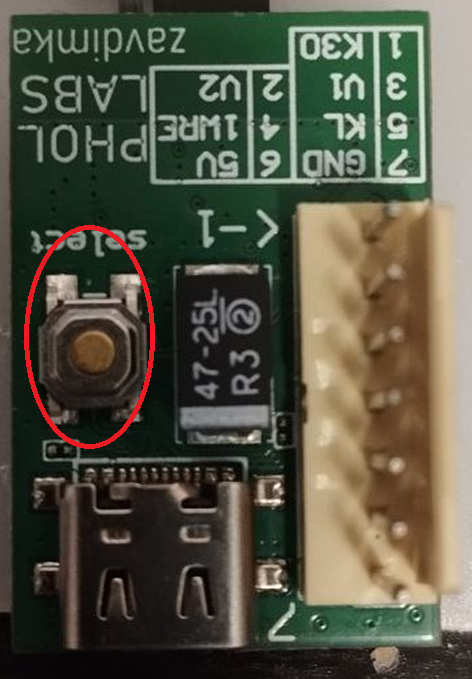
\includegraphics[width=.85\textwidth,height=.60\textheight,keepaspectratio]{figures/ivevo/image11.png}
\caption{Настройка Wi-Fi}
\end{figure}
